%%%%%%%%%%%%%%%%%%%%%%%%%%%%%%%%%%%%%%%%%%%%%%%%%%%%%%%%%%%%%%%%%%%%%%%%%%%%%%%%%%%%%%%%%%
\documentclass[runningheads]{llncs}                                                      %
%%%%%%%%%%%%%%%%%%%%%%%%%%%%%%%%%%%%%%%%%%%%%%%%%%%%%%%%%%%%%%%%%%%%%%%%%%%%%%%%%%%%%%%%%%

\usepackage{subfigure}
\usepackage{amssymb,amsmath}
\usepackage{graphicx}
\usepackage{array}
\usepackage{stmaryrd}
\usepackage{tikz}
\usepackage[draft]{hyperref}
\usepackage{listings}
\usepackage{cancel}
\usepackage[capitalize]{cleveref}
\usepackage{marginnote}

%%%%%%%%%%%%%%%%%%%%%%%%%%%%%%%%%%%%%%%%%%%%%%%%%%%%%%%%%%%%%%%%%%%%%%%%%%%%%%%%%%%%%%%%%%

\Crefname{figure}{Figure}{Figures}

%%%%%%%%%%%%%%%%%%%%%%%%%%%%%%%%%%%%%%%%%%%%%%%%%%%%%%%%%%%%%%%%%%%%%%%%%%%%%%%%%%%%%%%%%%

\newcommand{\MH}[2]{\marginnote{\tiny\color{red}(MH: #2)}\textcolor{red}{#1}}

%%%%%%%%%%%%%%%%%%%%%%%%%%%%%%%%%%%%%%%%%%%%%%%%%%%%%%%%%%%%%%%%%%%%%%%%%%%%%%%%%%%%%%%%%%
\begin{document}                                                                         %
%%%%%%%%%%%%%%%%%%%%%%%%%%%%%%%%%%%%%%%%%%%%%%%%%%%%%%%%%%%%%%%%%%%%%%%%%%%%%%%%%%%%%%%%%%

\title{ApiNATOMY: Towards Multiscale Views\\of Human Anatomy}

\author{
  Bernard de Bono\inst{2}
  \and
  Pierre Grenon\inst{2}
  \and
  Michiel Helvenstijn\inst{1}
  \and 	
  Joost Kok\inst{1}
  \and
  Natallia Kokash\inst{1}
  \fnmsep
  \thanks{Corresponding author, email: \email{nkokash@liacs.nl}}
}

\institute{
  Leiden Institute of Advanced Computer Science (LIACS), Leiden, The Netherlands
  \and University College London (UCL)
}

\maketitle

\setlength{\subfigcapskip}{0.1cm}
\setlength{\abovecaptionskip}{0cm}
\setlength{\belowcaptionskip}{0cm}
\setlength{\textfloatsep}{10pt plus 1.0pt minus 2.0pt}

%%%%%%%%%%%%%%%%%%%%%%%%%%%%%%%%%%%%%%%%%%%%%%%%%%%%%%%%%%%%%%%%%%%%%%%%%%%%%%%%%%%%%%%%%%

\begin{abstract}
Physiology experts deal with complex biophysical relationships, across multiple spatial and temporal scales.
Automating the discovery of such relationships, in terms of physiological meaning, is a key goal to the physiology community.
ApiNATOMY is an effort to provide an intuitive graphical interface for managing ontologies and semantic metadata relevant to physiology.
In this paper, we present a web-based ApiNATOMY environment for physiology experts to navigate through circuitboard visualizations of body components and their connections across scales. In particular, we present a tool prototype that visualizes schematics of ontology-based knowledge about body parts and their cardiovascular and neural connections. Graphical renderings of gene products and mathematical models of processes that are semantically annotated with this knowledge are overlaid on these schematics.
\end{abstract}

%%%%%%%%%%%%%%%%%%%%%%%%%%%%%%%%%%%%%%%%%%%%%%%%%%%%%%%%%%%%%%%%%%%%%%%%%%%%%%%%%%%%%%%%%%

%%%%%%%%%%%%%%%%%%%%%%%%%%%%%%%%%%%%%%%%%%%%%%%%%%%%%%%%%%%%%%%%%%%%%%%%%%%%%%%%%%%%%%%%%%
\section{Introduction}                                                                   %
%%%%%%%%%%%%%%%%%%%%%%%%%%%%%%%%%%%%%%%%%%%%%%%%%%%%%%%%%%%%%%%%%%%%%%%%%%%%%%%%%%%%%%%%%%

An ontology consists of a set of terms that represent a specific domain of knowledge, and their relations. They are created and maintained by knowledge domain experts, and are used as computer-readable taxonomies by software tools to support knowledge management activities in that domain.

The complexity of some of the ontologies in current use, as well as the complexity of handling semantic metadata that annotate third party resources with ontology terms (e.g. as described in~\cite{BHW+11}), has generated considerable demand for effective visualization in the design, authoring, navigation and management of (i) ontology-based knowledge and (ii) semantic metadata that uses ontologies.

In response to the above demand, a number of generic ontology visualization tools have been developed to assist knowledge acquisition, browsing and maintenance of ontologies~\cite{KHL+07}. Such tools, however, put considerable and unrealistic demands on the users' familiarity and expertise in both (i) semantic web technologies and (ii) the design principles of ontologies. It is unlikely that a user with expertise in the \emph{domain} of an ontology also has expertise in the \emph{technologies}.

The domain of biomedical physiology is a case in point. Physiology experts deal with complex biophysical operations, across multiple spatial and temporal scales, which they represent in terms of the transfer of energy from one form to another and/or from one anatomical location to another. Different kinds of descriptions of these biophysical operations are produced by different disciplines in biomedicine. For instance, (i) a medical doctor may describe the mechanism by which a stone in the ureter causes damage in the kidney; (ii) a pharmacologist may depict the process by which a drug absorbed from gut transits to the hip joints where it reduces inflammation; (iii) a molecular geneticist may trace the anatomical distribution of the expression of particular gene to understand the cause of a skeletal malformation; and, (iv) a bioengineer may build a mathematical model to quantify the effect of hormone production by the small intestine on the production of bile by the liver. These descriptions take diverse forms, ranging from images and free text (e.g., a paper in a journal) to XML documents bearing well-defined data or sets of variables and related equations (which could be used for as input for a simulation tool).

Automating the discovery of relationships, in terms of physiological meaning, between the above types of description is a key goal to the physiology community. To that end, this community is investing considerable effort in building ontologies for the annotation and semantic management of resources describing physiology. A number of reference ontologies have been created to represent the various entities required to describe physiology, including gene products~\cite{Bla+13}, chemical entities~\cite{HMD+13}, cells~\cite{BRA05} and gross anatomy~\cite{RM03}. Cumulatively, these reference ontologies consist of hundreds of thousands of terms, such that the volume of semantic metadata arising from annotation of resources with these terms is considerable. However, conventional technology for the management of ontologies and metadata is not usefully accessible to physiology experts.

The ApiNATOMY effort has emerged to provide intuitive graphical interface for managing ontologies and semantic metadata relevant to physiology. In this paper, we present a web-based ApiNATOMY environment for physiology experts to navigate through circuitboard visualizations of body components and their connections across scales. In particular, we present a tool prototype that visualizes schematics of ontology-based knowledge about body parts and their cardiovascular and neural connections. Graphical renderings of gene products and mathematical models of processes that are semantically annotated with this knowledge are overlaid on these schematics.

This paper is structured as follows: first, we give an overview of the ontology, metadata and data resources that we focus on, and outline usage scenarios that motivate our work (\cref{sect:motivation}).  We then we discuss representation and visualization methods applied to arrange and display relevant resources (\cref{sect:visualization,sect:visualization2}). In \cref{sect:implementation}, we describe the graphical tool prototype that implements these methods. Furthermore, in \cref{sect:relatedWork}, we overview related methodologies, efforts and techniques in the field. Finally, we conclude the paper and discuss future work in \cref{sect:conclusions}.

%%%%%%%%%%%%%%%%%%%%%%%%%%%%%%%%%%%%%%%%%%%%%%%%%%%%%%%%%%%%%%%%%%%%%%%%%%%%%%%%%%%%%%%%%%
\section{Use Case, Resources and Early-stage Results} \label{sect:motivation}            %
%%%%%%%%%%%%%%%%%%%%%%%%%%%%%%%%%%%%%%%%%%%%%%%%%%%%%%%%%%%%%%%%%%%%%%%%%%%%%%%%%%%%%%%%%%

In this section, we briefly discuss core use cases for the ApiNATOMY application: schematics in support of genomics and drug discovery studies. In so doing, we introduce (i) some of the key ontological and data resources required in this case, as well as (ii) early-stage results of the ApiNATOMY application effort.

The domains of genomics and drug discovery are dependent on physiology knowledge, as both domains take into account the manufacture of gene products in different parts of the body and the regulated long-distance transport of molecules that interact with these products. The location of gene product manufacture (i.e. gene expression data, such as~\cite{EBI}), as well as routes associated with pharmacokinetic modeling of molecular interactors (drawn from resources such as~\cite{HMC+13}) may be usefully depicted in the form of a physiology \emph{circuitboard}.

In ApiNATOMY, a physiology circuitboard schematic consists of a combination of (i) an anatomical treemap and (ii) an overlay of process graphs. In our earlier prototypes (described in~\cite{BGS12,KBK14}), templates were applied to constrain the layout of tiles in treemaps of the Foundational Model of Anatomy (FMA)~\cite{RM03} ontology, such that nesting of one tile inside another indicates that the child tile is either a \emph{part} or a \emph{subclass} of the parent tile. The Graphical User Interface (GUI) providing the interaction with the circuitboard allows point-and-click navigation of the treemap content. This type of interaction extends to also to involve process graphs - in this paper we report on the graphical projection of routes of (i) blood flow processes linking different regions of the human body (using data generated in~\cite{deB11}), as well as (ii) transport processes along neurons of the central nervous system (i.e. brain and spinal cord) with data obtained via the Neuroscience Information Framework~\cite{Gar+08}.

The ApiNATOMY Graphical User Interface is built from inception as a three dimensional (3D) environment. This facilitates interaction not only with 3D renderings of the circuit boards themselves, but also with a wide range of geometry/mesh formats for volumetric models of biological structure across scales. For instance, it is already possible to overlay Wavefront .obj data from BodyParts3D~\cite{MFT+09} as well as SWC data provided by neuromorpho.org~\cite{Asc06}.
% TODO: acknowledge the contribution of SharkViewer to our rendering of .swc files
% Sharkviewer: https://github.com/JaneliaSciComp/SharkViewer
% Janelia Farm research campus: http://www.janelia.org
% SWC File Format Specification: http://research.mssm.edu/cnic/swc.html
% I have asked the SharkViewer people how they'd like to be cited: https://github.com/JaneliaSciComp/SharkViewer/issues/4

In the following sections, we discuss:
\begin{itemize}
  \item the constraining of treemap layouts to generate stable anatomical treemaps,
  \item the design and overlay of communication routes for the cardiovascular and neural systems, and
  \item the querying and 3D depiction of protein architecture schematics for the anatomical overview of gene expression data.
\end{itemize}

\begin{figure}
	\centering
	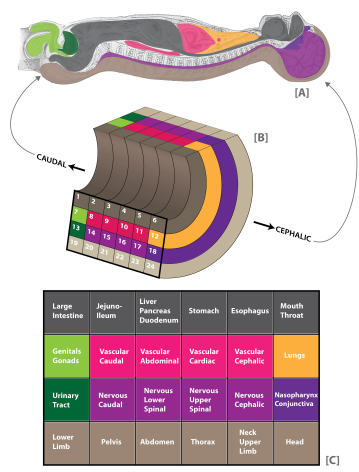
\includegraphics[width=6cm]{images/application.png}
	\caption{Longitudinal section through the middle of the male human body}
	\label{fig:application}
\end{figure}
%	\subfigure[Visualizing medical ontologies using treemaps]{
%		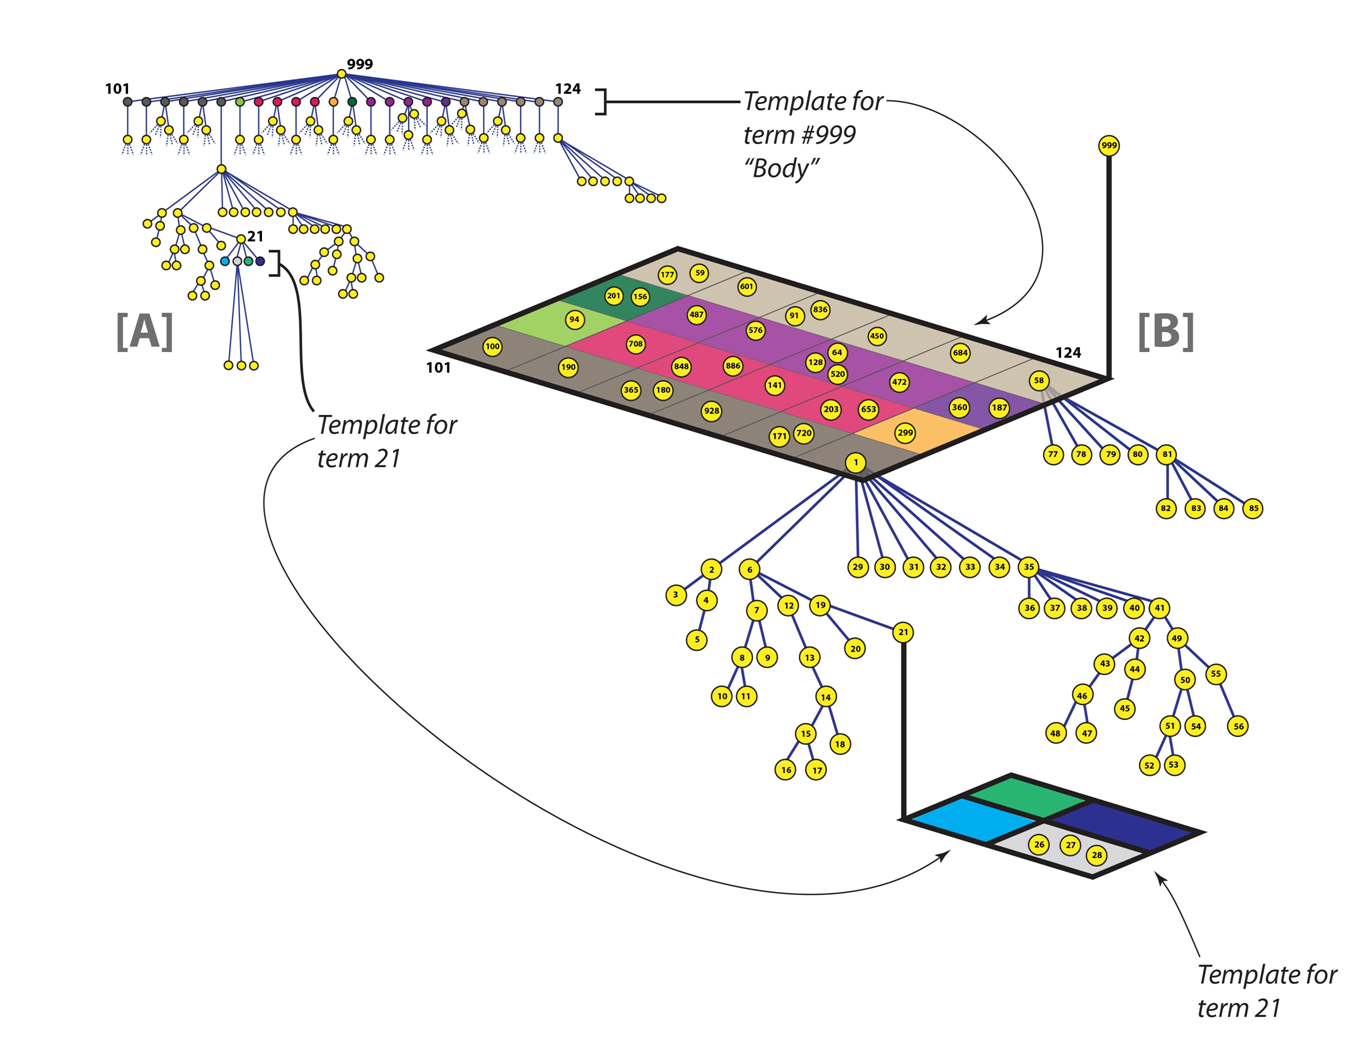
\includegraphics[width=7.3cm]{images/application1.png}
%	}

We arrange data in a hierarchical structure, starting from the large-scale views of external and internal surfaces and organs.
This upper level is arranged to resemble the longitudinal section through the middle of the human body (\cref{fig:application}).
Each of the organs in the plan is composed of multiple tissues and sub-organs, the structural information about them is obtained from the FMA ontology~\cite{RM03}. The tool to support data filtering across multiple levels and contextual zooming into selected areas.
% TODO: refer to other figure

%%%%%%%%%%%%%%%%%%%%%%%%%%%%%%%%%%%%%%%%%%%%%%%%%%%%%%%%%%%%%%%%%%%%%%%%%%%%%%%%%%%%%%%%%%
\section{Visualizing Taxonomies and Connectivity Data} \label{sect:visualization}        %
%%%%%%%%%%%%%%%%%%%%%%%%%%%%%%%%%%%%%%%%%%%%%%%%%%%%%%%%%%%%%%%%%%%%%%%%%%%%%%%%%%%%%%%%%%

Treemaps~\cite{JS91} are an effective technique to visualize hierarchical data by using nested shapes in a space-filling layout.
Each shape represents a geometric region, which can be subdivided recursively into smaller regions. The standard shape is a rectangle.
Nodes in a treemap, also called \emph{tiles}, represent individual data items in a dataset. Node size, color and text label can be used to represent attributes of the data item. One-layered treemaps can display data attributes but are not very good at emphasizing the place of an item in the overall hierarchical structure. To compensate for that, a small margin with structural labels is typically used. In treemaps displaying hierarchical structures, it is possible to navigate among different layers and zoom into selected tiles~\cite{BL07}.

% TODO: rewrite the 'flat treemap' text for a bit of extra clarity (MH)

To create a treemap, one must define a tiling algorithm - a way to divide a tile into sub-tiles of specified areas.
Tiling algorithms used for typical applications of treemaps such as e.g., visualization of folders in files in the computer file system with their respected sizes, do not associate tile positions with any characteristic of the data. This is not the case in our scenario: while a user navigates among different layers, filters data and zooms into selected areas, the tiles should be kept in the same relative positions to each other. Otherwise, the user's perception of the displayed information will be quickly disrupted. Moreover, our tiling algorithm should allow the user to enforce constraints on tile positions to make the treemap views structurally resemble body regions. Hence, we developed a stable and customizable tiling algorithm that arranges tiles according to a given template~\cite{KBK14}.

For a set of $n$ data items with no positional constraints, a default template is created that consists of $\lfloor \sqrt{n}\, \rfloor$ rows and $\lceil \sqrt{n}\, \rceil$ columns in each row but the last one (which may contain fewer columns). If the positional data is available (e.g., FMA ontology adjacent-to relation) or a user wants to rearrange the data manually, a custom template is associated with the parent node of the dataset items. The template is a hierarchical structure
$\bigl\{\mathit{splitType}, \{\},\ldots, \{\}\bigr\}$ where $\mathit{splitType} \in \left\{\mathrm{slice}, \mathrm{dice}\right\}$ defines a way to split the rectangle into sub-rectangles: vertically or horizontally. By recursively splitting the available area into sub-rectangles, one can define complex layouts that enforce two dimensional constraints in the form ``$x$ is left/right of $y$'' or ``$x$ is above/below of $y$'' where $x$ and $y$ are individual data items or groups of data items that in their turn can be allocated as needed using the same technique.

The schematic body plans created using template-based treemaps can be seen in \cref{fig:treemaps}. \Cref{fig:24tiles} shows the top level 24 tile body anatomy plan. The choice of this layout is explained by \cref{fig:tilemap-cylinder}, which shows how it can conceptually wrap around the longitudinal axis of the human body. The treemap layout is controlled by the (default) templates and remains stable during navigation.


\subsection{Connectivity data} %%%%%%%%%%%%%%%%%%%%%%%%%%%%%%%%%%%%%%%%%%%%%%%%%%%%%%%%%%%

With the treemap-based body plans as background, we overlay the schematic representation of \emph{body systems} such as circulatory, respiratory, or nervous systems. Body systems are essentially graphs with nodes corresponding to body parts (treemap tiles) or entities inside of body parts (proteins, cells, etc.), and their edges represent organ system compounds such as blood vessels or nervous connections that pass through such body parts or sub-parts.
%%
They may also contain auxiliary nodes that are not represented on the treemap but still carry important biomedical information.

Body systems are intrinsically complex and require efficient data visualization techniques to help avoid clutter induced by the large amount of graph edges and their crossings. To support the GUI functionality, body systems must allow users to overview large parts of the body systems as well as to trace individual connections and analyze their structure. In this context, edge bundling techniques~\cite{Hol06,GHN+11,HET12} have been proposed to improve perception of connectivity data in large dense graphs. Such techniques generally rely on edge rerouting strategies that are either solely targeted at improving visual perception (by using the positions of nodes) or exploit the relationships among connectivity data as guidelines for a more natural allocation of graph edges and nodes. Our application requires a mixture of these techniques.

As an example, consider the schematic visualization of blood vessels in human body. Our initial dataset is a graph based on the FMA resource, and consists of approximately 11,300 edges and over 10,000 distinct nodes. In this graph, an edge represents a flow process over an unbranched segment of a blood vessel. Nodes represent blood vessel junctions and end-points. Samples of records from the dataset are shown in \cref{tab:vascular-connectivity}. The first column in the dataset is a unique vascular segment identifier (ID), the second column bears the biological type of segment (1 - for arterial segment, 2 - microcirculation (MC), 3 - venous, and 4 - cardiac chamber), the third represents FMA IDs, the fourth and fifth are unique node identifiers in an edge pair, and the last column is a free-text description.

\begin{table}
\caption{Vascular connectivity data from the FMA ontology}
\begin{tabular}{|l|l|l|l|l|p{7cm}|}
  \hline
  Segment & Type & FMA & Node 1 & Node 2 & Description \\
  \hline
  121a & 2 & 62528 & 62528\_2 & 62528\_4 & Arterioles in Microcirculation segment of Wall of left inferior lobar bronchus \\
  121c & 2 & 62528 & 62528\_4 & 62528\_5 & Capillaries in Microcirculation segment of Wall of left inferior lobar bronchus\\
  121v & 2 & 62528 & 62528\_3 & 62528\_5 & Venules in Microcirculation segment of Wall of left inferior lobar bronchus\\
  ... &... & ...   & ...      & ...      & ...\\
  8499 & 1 & 69333 & 8498\_0 & 62528\_2  & Arterial Segment 8499 of Trunk
of left second bronchial artery from origin of supplying terminal segment
to the arteriolar side of the Wall of left inferior lobar bronchus
MC\\
  9547 & 3 & 66699 & 9546\_0 & 62528\_3 & Venous Segment 9547 of Trunk of
left bronchial vein from origin of supplying terminal segment to the
venular side of the Wall of left inferior lobar bronchus MC \\
  \hline
\end{tabular}
\label{tab:vascular-connectivity}
\end{table}

An MC is represented by three edges connected in series: one edge represents tissue arterioles, a second edge stands for the bed of
capillaries, while a third denotes the venules. In one MC, therefore: a) the end node of the arteriolar edge and the start node of the
capillary edge are equivalent, and b) the end node of the capillary edge and the end node of the venular edge are equivalent.

In the above example, the anatomical entity in which the MC is embedded is 62528 - the topology of MC segment connectivity is as follows:
\[
	62528\_2  \;\xrightarrow{\;\text{121a}\;}\;
	62528\_4  \;\xrightarrow{\;\text{121c}\;}\;
	62528\_5  \;\xleftarrow {\;\text{121v}\;}\;
	62528\_3  \text.
\]
MC segment 121a is supplied with blood by the arterial segment 8499 while MC segment 121v is drained of blood by the venous segment 9547.

The accurate visualization of the cardiovascular system in a comprehensible way requires complex pre-processing (about 12 rules were identified to extract the data of interest from the presented dataset by a biomedical expert in our team).
In this paper, for illustration purpose we show only paths connecting MCs of the walls of the heart (i.e., wall of left ventricle (FMA ID 7101), left atrium (7097), right ventricle (7098) or right atrium (7096)) to MCs belonging to the sub-organs of the organs in our upper level 24 tile body plan.
To obtain this view, we looked for the shortest paths (due to the way the data is represented in the initial data set, cycles are possible) from the MCs of the heart walls to the final FMA tiles. For example, the path from the left ventricle to the wall of left inferior lobar bronchus MC looks like
{$7101 \rightarrow 2406 \rightarrow \cdots \rightarrow 8499 \rightarrow 62528$,}
while the path from this organ to the right atrium is like follows:
{$7096 \leftarrow 771 \leftarrow \cdots \leftarrow 9546 \leftarrow 9547 \leftarrow 62528$.}

The first and the last IDs in this path correspond to the tiles in the treemap, while the intermediate IDs will be represented using auxiliary nodes with undefined coordinates. One of the issues we encountered is the need to determine optimal positions for these nodes. Since several paths as above can have common sub-paths, the intermediate nodes should not deviate too much from the way from the heart MC to each of the end tiles sharing such sub-paths. This motivates our application of the sticky force-directed graph visualization method~\cite{FR91,Bos14} in which a sub-set of nodes have fixed coordinates, and the coordinates of the other nodes is determined by simulating imaginary forces applied by their edges (\cref{fig:bloodvessels}).
%%%% (MH: seems like an implementation detail)
% As our only objective is to allocate intermediate nodes as close to the
% paths they belong to (which most naturally can be represented by straight
% lines) as possible, we set gravity and charge to 0 and the desired link
% length to a minimal possible length.
%%%%

If there are too many edges to get a clear overview of the data ---as in \cref{fig:force-7101},
which shows the full connectivity graph for the left ventricle (7101) on the top-level body plan---
we can apply a hierarchical edge bundling method that uses the path structure to bundle common sub-paths.
The result for the left ventricle is shown in \cref{fig:bundled-7101}, which gives a much nicer
overview. The result for the right atrium is shown in \cref{fig:bundled-7096}.
%%%% (MH: seems like an implementation detail)
% By setting bundling algorithm tension parameter close to 1 (0.96-0.99),
% we obtain a view that clearly shows that individual paths extracted from
% our dataset form ``highways'' which correspond to major arteries and
% veins in the human body.
%%%%
\begin{figure}[h]%
  \centering%
  \subfigure[Selected blood vessel connections]{
    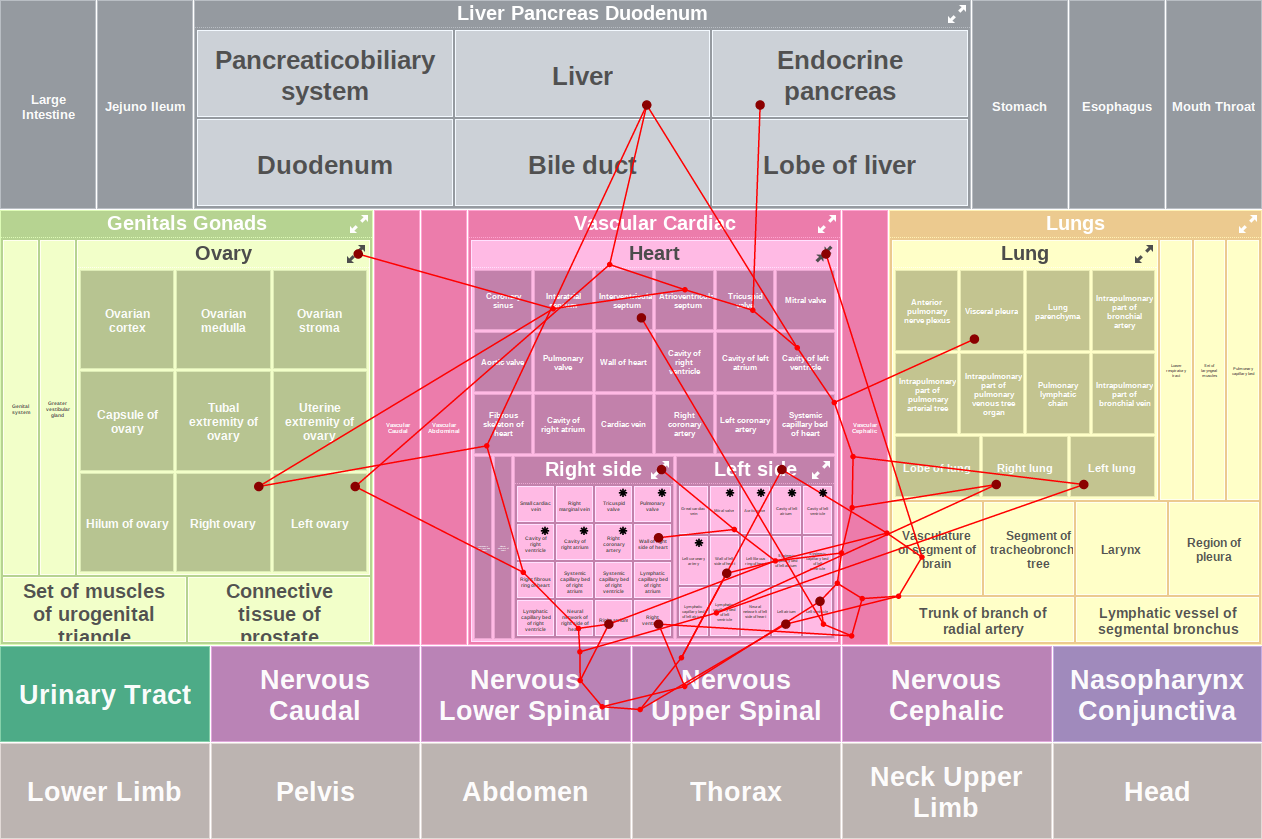
\includegraphics[width=5.8cm]{images/screenshot-bloodvessels.png}
    \label{fig:bloodvessels} % TODO: refer to this
  }%
  \subfigure[Arterial connections from left ventricle]{
    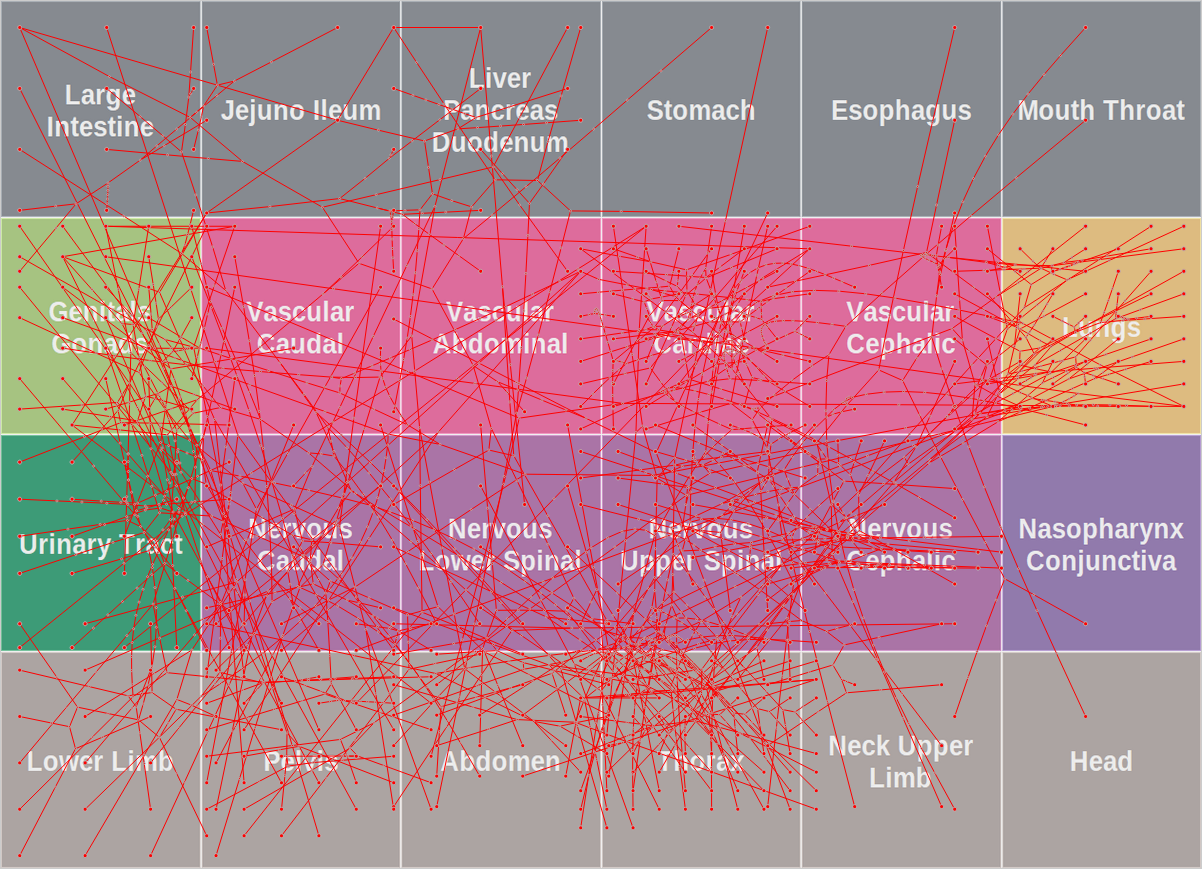
\includegraphics[width=5.8cm,height=3.855cm]{images/force-7101-new.png}
    \label{fig:force-7101}
  }\vskip-2mm
  \subfigure[Bundled paths from left ventricle]{
    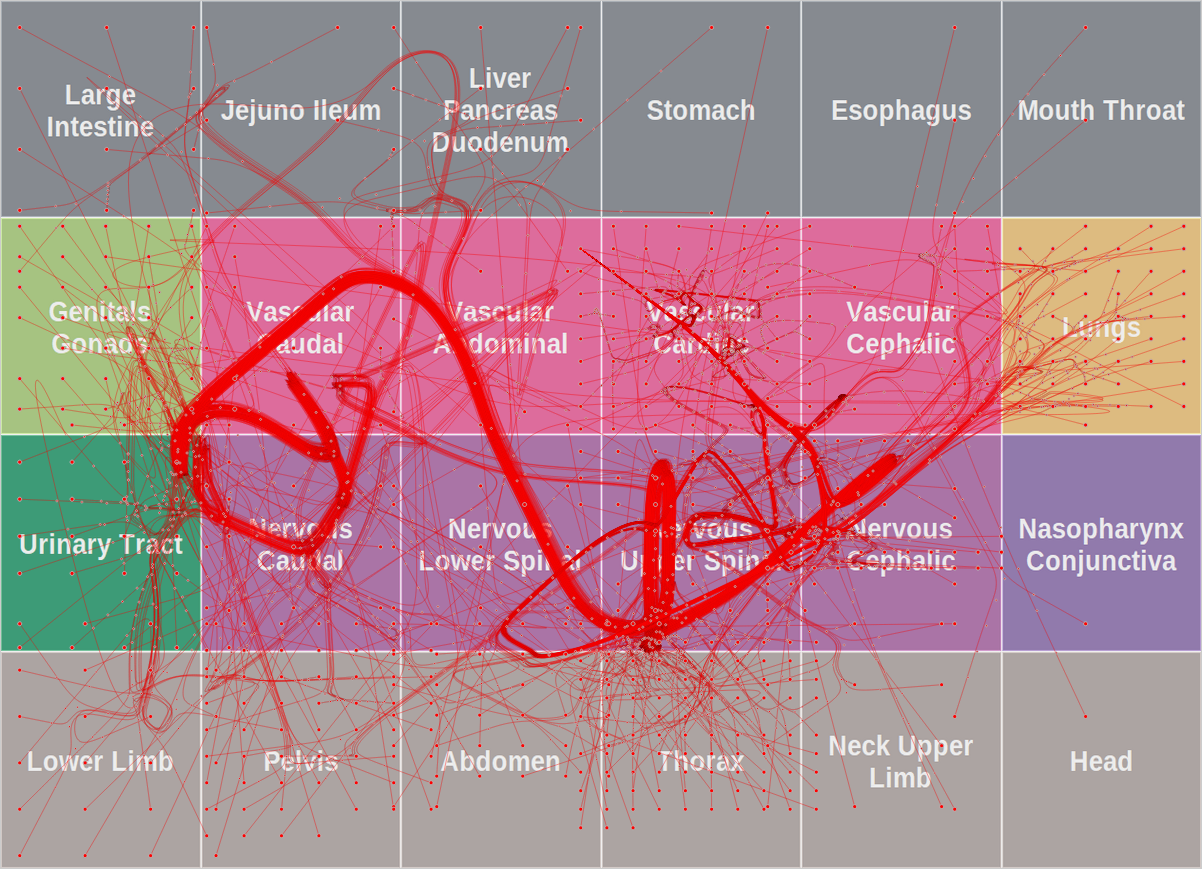
\includegraphics[width=5.8cm,height=3.855cm]{images/connections-7101-new.png}
    \label{fig:bundled-7101}
  }%
  \subfigure[Bundled paths to right atrium]{
    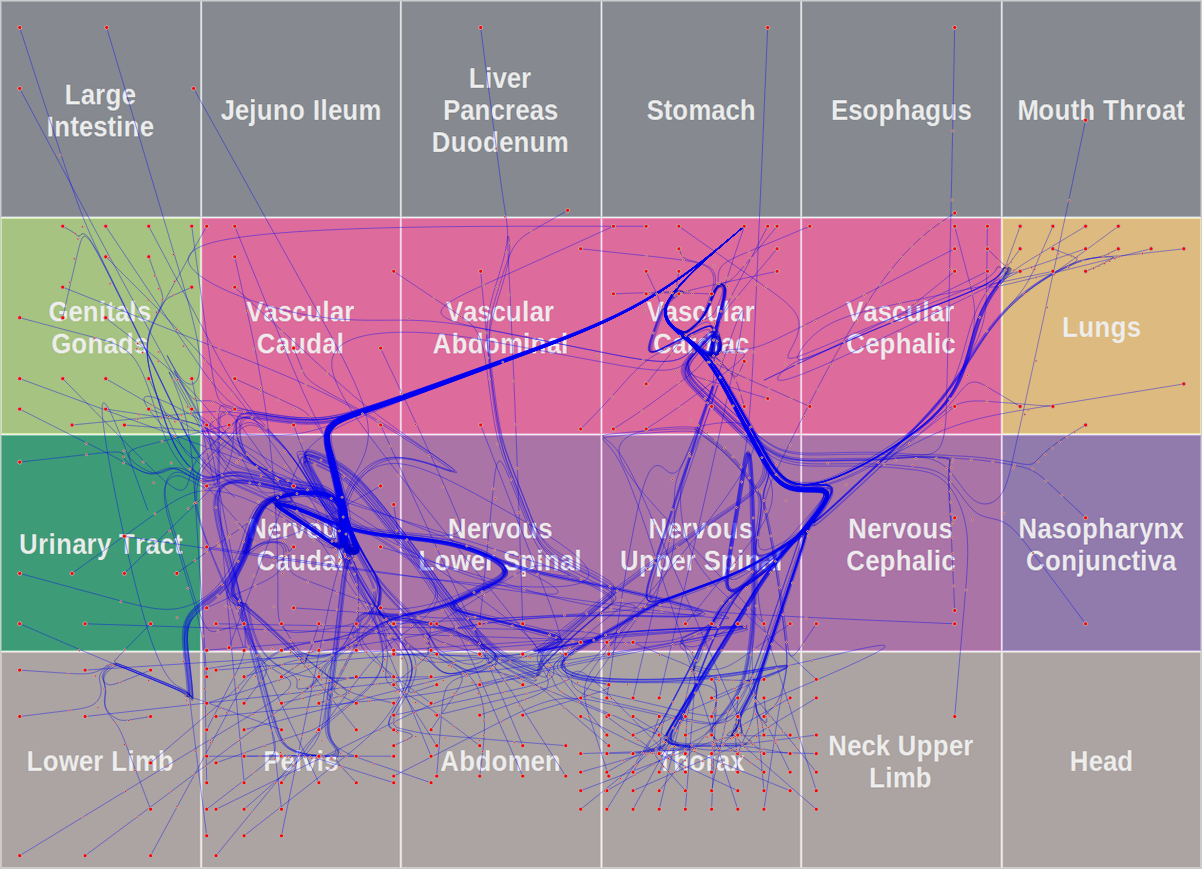
\includegraphics[width=5.8cm,height=3.855cm]{images/connections-7096b-new.png}
    \label{fig:bundled-7096}
  }\vskip1mm
  \caption{Cardiovascular system}
  \label{fig:vascular-connectivity}
\end{figure}

After a one-time pre-processing to import data from available external sources, we store connectivity data in a convenient format. A user can interact with and edit this data using our application.

One of the prime goals of the tool is to simplify the access and maintenance of biomedical taxonomies, including those concerned with physiological connectivity data. A user should be able to customize the way in which that data is represented. There is ongoing work on an implementation of the orthogonal connector visualization algorithm that would place edges into margins between tiles so that they will not obstruct the interaction with the tiles themselves.


%%%%%%%%%%%%%%%%%%%%%%%%%%%%%%%%%%%%%%%%%%%%%%%%%%%%%%%%%%%%%%%%%%%%%%%%%%%%%%%%%%%%%%%%%%
\section{Visualization of Models and Metadata} \label{sect:visualization2}               %
%%%%%%%%%%%%%%%%%%%%%%%%%%%%%%%%%%%%%%%%%%%%%%%%%%%%%%%%%%%%%%%%%%%%%%%%%%%%%%%%%%%%%%%%%%

The entities in the ApiNATOMY ontologies have various data associated with them, to which they are explicitly linked via semantic metadata annotations. This includes, for instance, static and dynamic 3D models of body organs and their subsystems.
To illustrate the application of ApiNATOMY in the management of semantic metadata and associated resources, we extract and display neuronal reconstructions and associated metadata from \url{http://neuromorpho.org}~\cite{Asc06}.
\Cref{fig:neuron-big} shows a sample neuron model associated with the neocortex (reached through``Nervous Cephalic'' $\rightarrow$ ``Region of cerebral cortex'' $\rightarrow$ ``Neocortex''). ApiNATOMY allows users to show multiple 3D objects together in their proper context. For example, \cref{fig:neuron-small} shows a screenshot of a circuit board with the ``Neocortex'' neuron, as well as 3D models of the ``Liver'' and ``Stomach''.

\begin{figure*}
\centering
  \subfigure[Neuron in the ``Neocortex'']{
    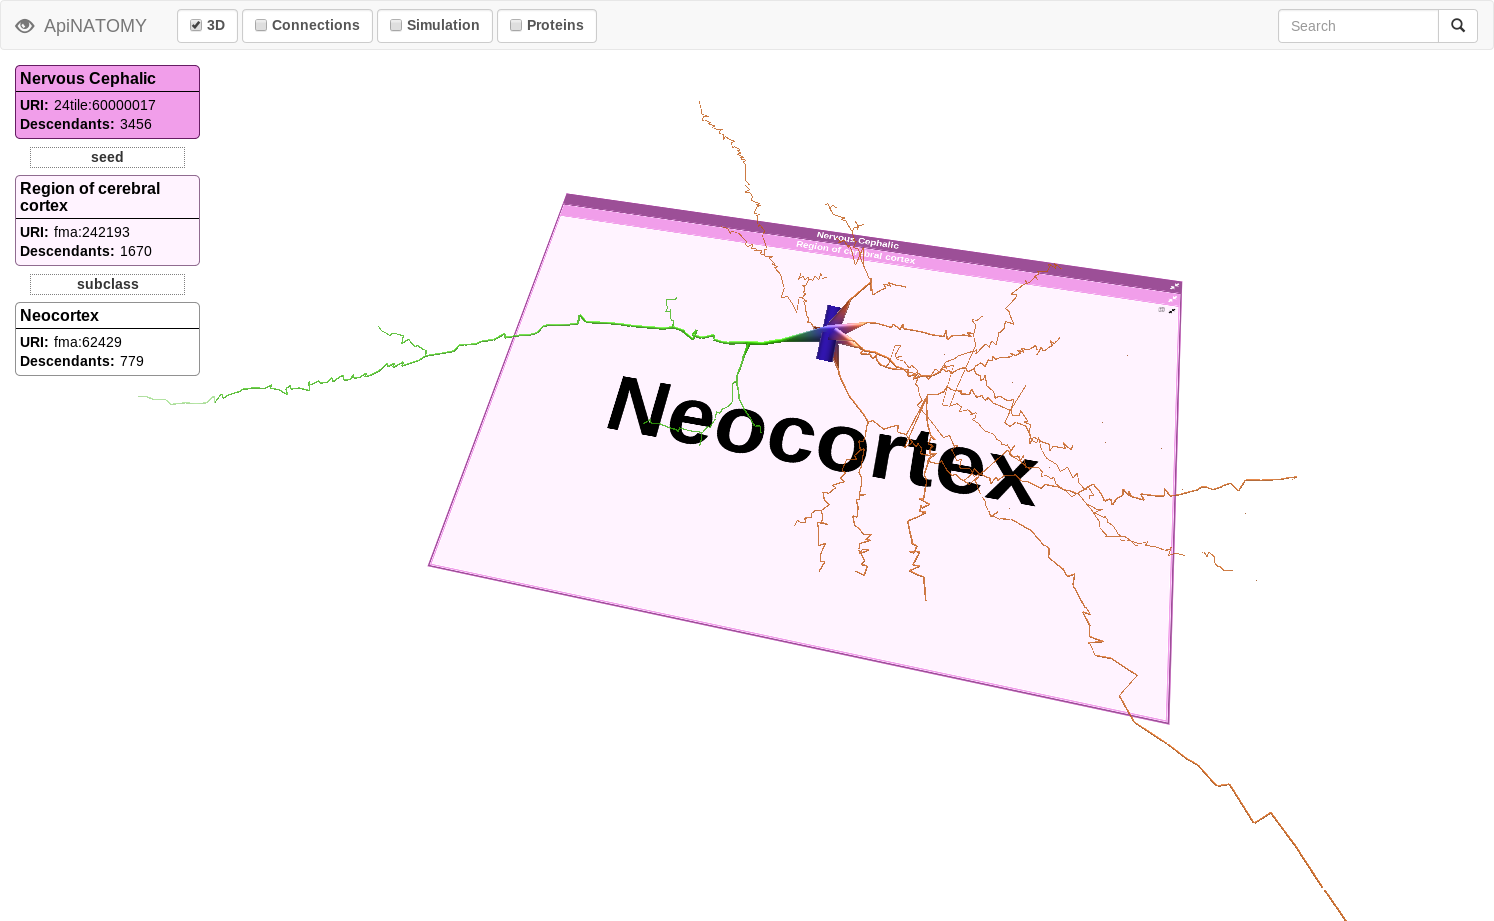
\includegraphics[width=5.4cm]{images/screenshot-neocortex-neuron.png}
    \label{fig:neuron-big}
  }
  \subfigure[Multiple 3D models in context]{
    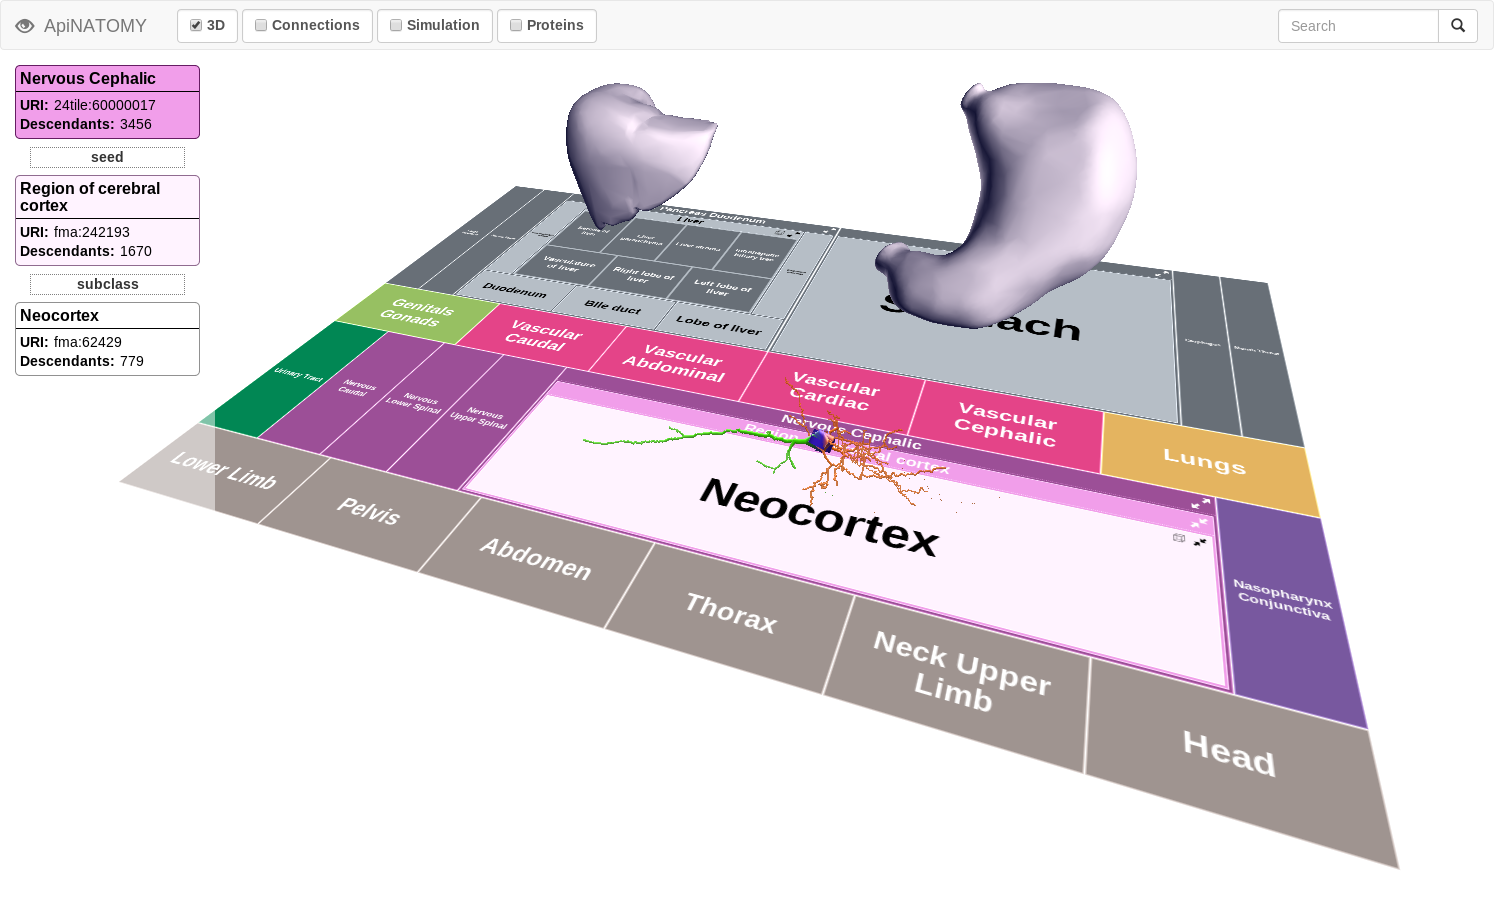
\includegraphics[width=5.4cm]{images/screenshot-3d-objects.png}
    \label{fig:neuron-small}
  }\vskip2mm
  \caption{Visualization of static 3D models}
  \label{fig:neurons}
\end{figure*}

ApiNATOMY also supports the visualization of protein- and drug-interaction networks (\cref{fig:protein}) that are represented as graphs on top of treemap tiles. We are in the process of acquiring and integrating relevant data from the Ensembl genomic database~\cite{Ensemble}. In Ensembl, gene models are annotated automatically using biological sequences data (e.g. protein, mRNA). We query this database to extract genes, transcripts, and translations with related protein features such as e.g., PFAM domains, and locate automatically-generated diagrams of proteins with FMA tiles to represent the anatomical location in which they are expressed. For ease of visualisation, protein diagrams show domain features built from different shapes and colors in a navigable 3D environment (\cref{fig:protein-3d}).

\begin{figure*}
\centering
%	\subfigure[Simulation control panel]{
%		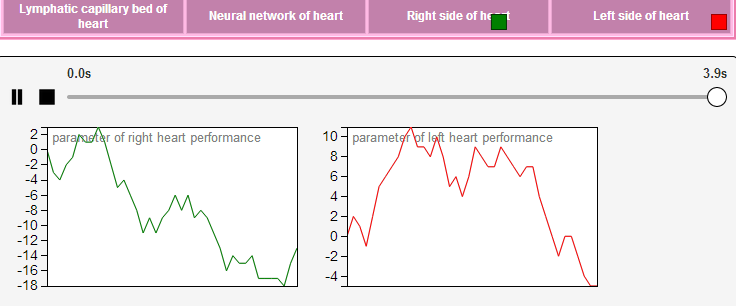
\includegraphics[width=5cm]{images/simulation.png}
%		\label{fig:panel}
%	}
	\subfigure[Protein interactions in 2D]{
		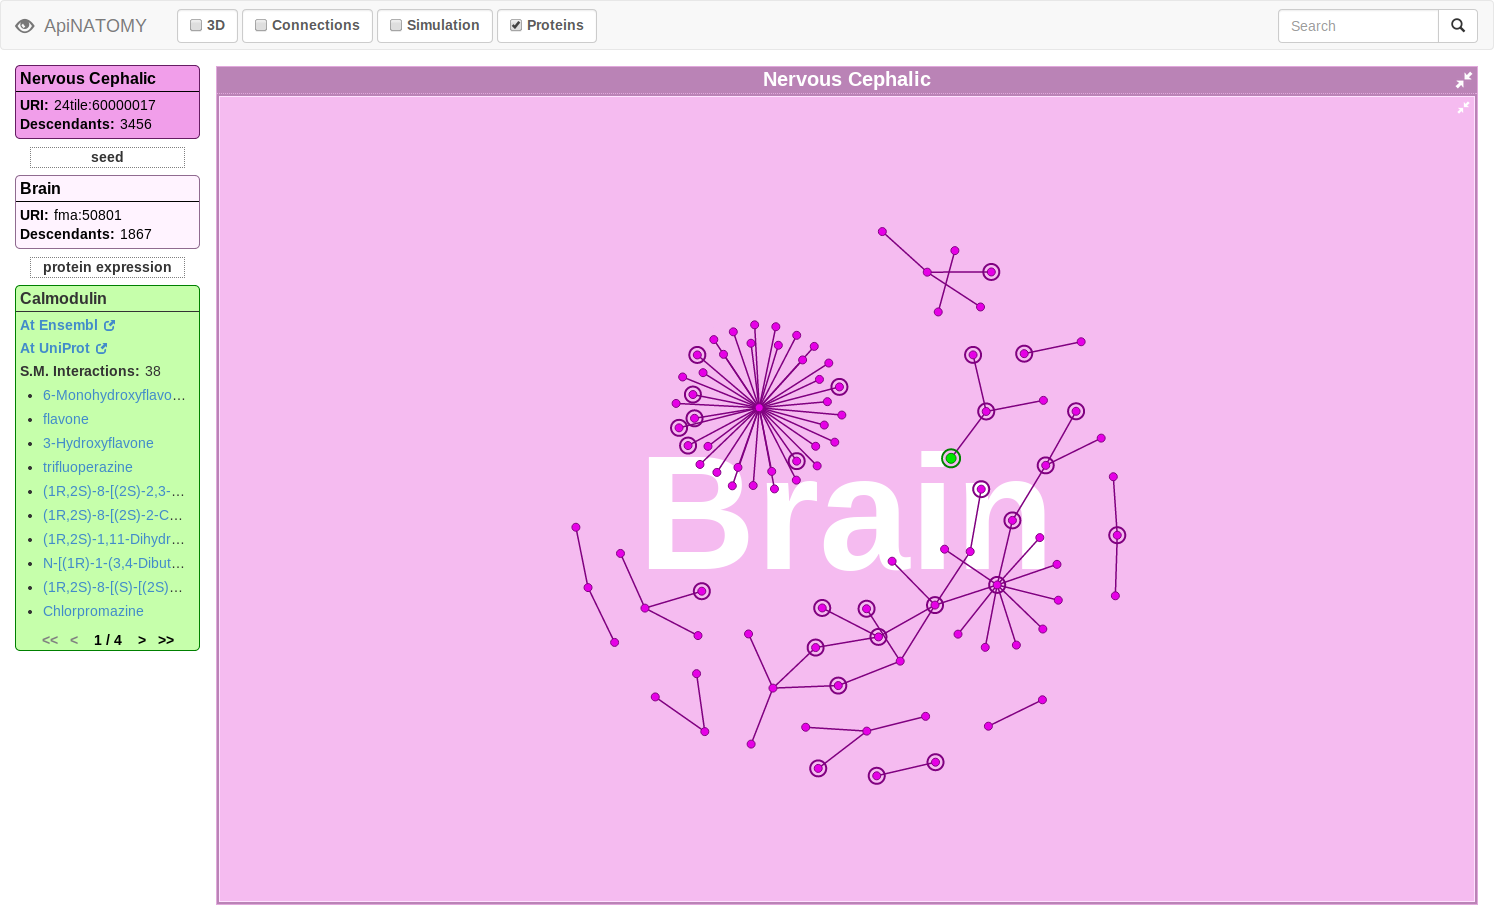
\includegraphics[width=5.4cm]{images/screenshot-proteins.png}
		\label{fig:protein}
	}
	\subfigure[Protein features in 3D]{
		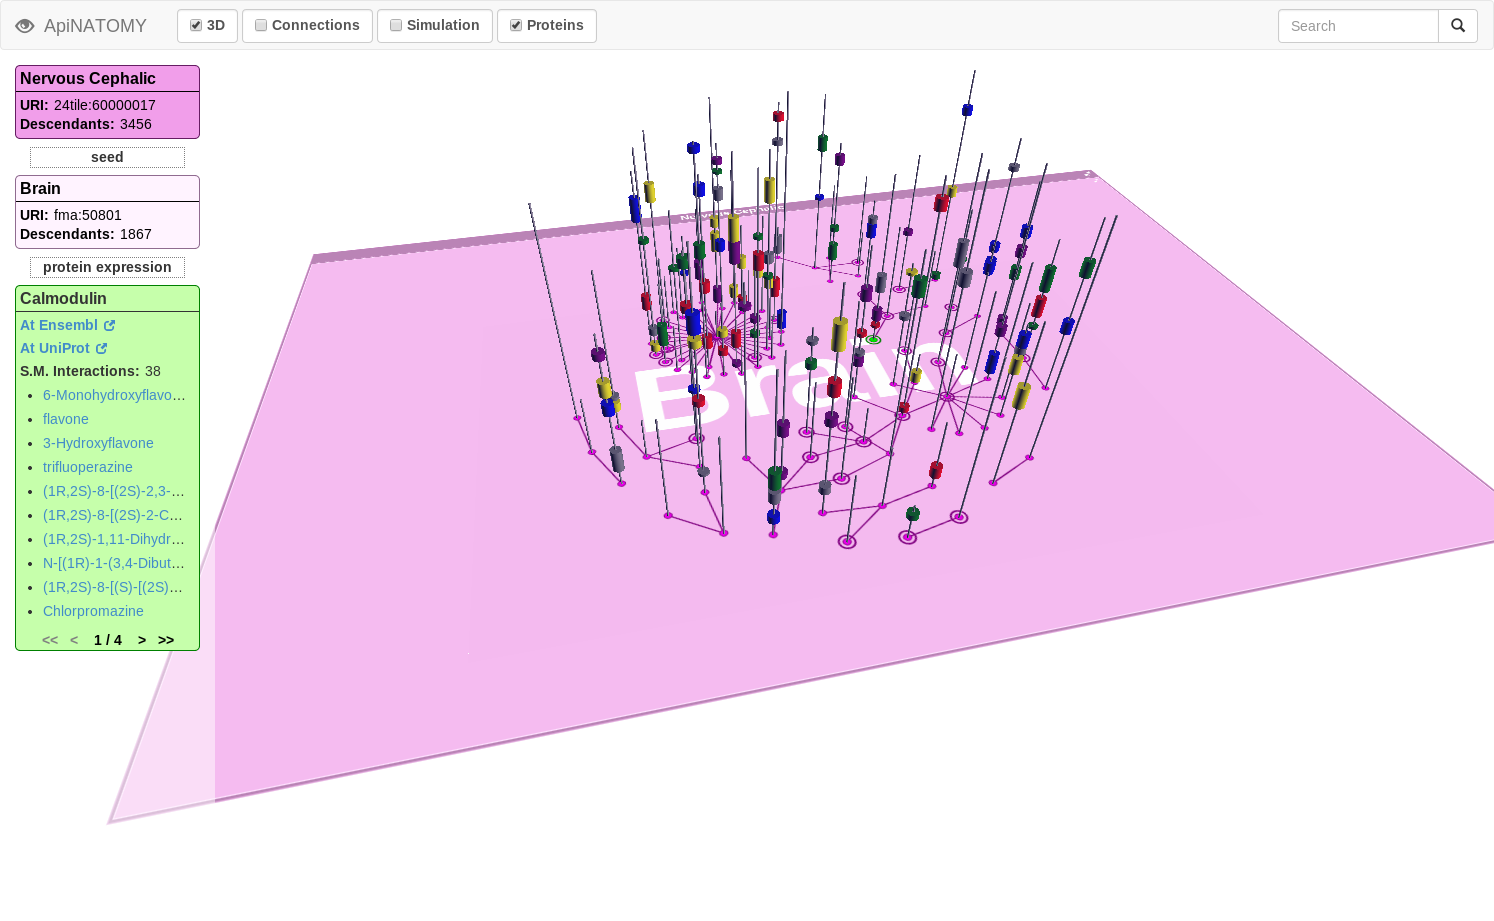
\includegraphics[width=5.4cm]{images/screenshot-proteins-3d.png}
		\label{fig:protein-3d}
	}
	\caption{Visualizing protein expression, protein interaction and protein features}
	\label{fig:proteins}
\end{figure*}

%%%%%%%%%%%%%%%%%%%%%%%%%%%%%%%%%%%%%%%%%%%%%%%%%%%%%%%%%%%%%%%%%%%%%%%%%%%%%%%%%%%%%%%%%%
\section{Implementation} \label{sect:implementation}                                     %
%%%%%%%%%%%%%%%%%%%%%%%%%%%%%%%%%%%%%%%%%%%%%%%%%%%%%%%%%%%%%%%%%%%%%%%%%%%%%%%%%%%%%%%%%%

\begin{figure}[ht]
	\centering
	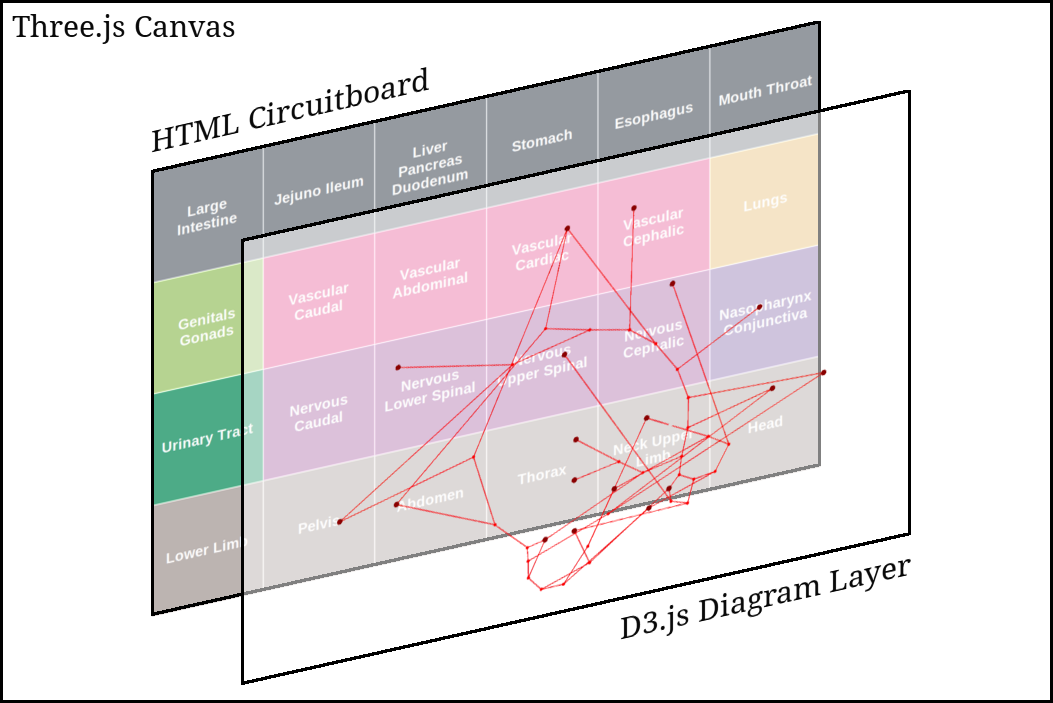
\includegraphics[width=6cm]{images/visual-layers.png}
	\hskip1mm
	\begin{tabular}[b]{lcl}
		\multicolumn{3}{l}{\textbf{Able to Control Position:}}     \\[1mm]
		Three.js Canvas     & $\longrightarrow$ & HTML Treemap     \\[1mm]
		Three.js Canvas     & $\longrightarrow$ & D3.js Layer      \\[3mm]
		
		\multicolumn{3}{l}{\textbf{Able to Add Content:}}          \\[1mm]
		HTML Treemap        & $\longrightarrow$ & D3.js Layer      \\[1mm]
		HTML Treemap        & $\longrightarrow$ & Three.js Canvas  \\[1mm]
		D3.js Layer         & $\longrightarrow$ & Three.js Canvas  \\[3mm]\vphantom{x}%hack
	\end{tabular}
	\vskip1mm
	\caption{The three layers of circuitboard visualization and their interaction.}
	\label{fig:visual-layers}
\end{figure}

In this section we discuss a number of implementation aspects of \mbox{ApiNATOMY}.
For maximum compatibility across operating systems as well as handheld devices,
the whole application is written in Javascript. The main framework in use is
AngularJS, which provides a Model-View-Controller architecture, as well as
two-way databinding. Connectivity- and protein-protein
interaction diagrams~(\cref{fig:vascular-connectivity,fig:protein})
are generated using D3.js, and all 3D functionality~(\cref{fig:neurons,fig:protein-3d})
is implemented using Three.js, which provides a convenient abstraction layer over WebGL.



%\subsection{Circuitboard Layers} %%%%%%%%%%%%%%%%%%%%%%%%%%%%%%%%%%%%%%%%%%%%%%%%%%%%%%%%%

The circuit-board is rendered with essentially three layers,
which are shown in \cref{fig:visual-layers}. The treemap is generated
with plain HTML. On top of this, a partly transparent diagram layer is
rendered by D3.js. The positions of the tiles and the positions of the
diagram nodes are synchronized with AngularJS two-way databinding.
When 3D mode is activated, Three.js takes control of both layers.
Besides rendering 3D objects with WebGL, it can manipulate HTML
elements using CSS 3D transforms. When using both rendering engines
in conjunction, Three.js can keep WebGL and HTML perfectly synchronized.
Together with AngularJS two-way databinding, we get very fine control
of positioning. This is demonstrated particularly well in \cref{fig:protein-3d}.
%%
To render \texttt{.swc} neuron files (\cref{fig:neurons}), ApiNATOMY uses SharkViewer,
an open source Three.js library
developed by the Howard Hughes Medical Institute~\cite{weaver_sharkviewer_2014}.

%\subsection{Focus and Direct Feedback} %%%%%%%%%%%%%%%%%%%%%%%%%%%%%%%%%%%%%%%%%%%%%%%%%%%

A separate module keeps track of the entity under focus. Whenever the mouse hovers
over a specific tile or object, it is highlighted and its hierarchical information
is shown in the left side-panel~(\cref{fig:neurons,fig:proteins}). Clicking on the object
fixes this focus, allowing the user to interact with the information in the side-panel.

This direct feedback has another purpose. An ontology need not necessarily be a
tree. In the FMA ontology, for example, different branches may join, making it a
directed acyclic graph. A treemap, however, by its very nature, is only suitable
for visualizing trees. We compensate for this by allowing the same entity to be
represented by more than one tile at the same time. To reinforce this intuition, all
such tiles are highlighted in unison when the mouse hovers over any one of them.
Only one tile per entity is considered `active'. Only the active tile may be opened
up to show its children, and only the active tile participates in the visualization
of cross-tile connectivity data.

%%%%%%%%%%%%%%%%%%%%%%%%%%%%%%%%%%%%%%%%%%%%%%%%%%%%%%%%%%%%%%%%%%%%%%%%%%%%%%%%%%%%%%%%%%
\section{Related work} \label{sect:relatedWork}                                          %
%%%%%%%%%%%%%%%%%%%%%%%%%%%%%%%%%%%%%%%%%%%%%%%%%%%%%%%%%%%%%%%%%%%%%%%%%%%%%%%%%%%%%%%%%%

The need for the multi-scale visualization and analysis of human body systems is well recognized by biomedical communities. For example,
3D Multiscale Physiological Human initiative deals with the mixtures of physiological knowledge and computational approaches to help scientists in biomedicine to improve diagnostics and treatments of various disorders~\cite{MRC09},\cite{Mag09}.
Numerous taxonomies and databases have been created and are widely used by researchers in the biomedical field~\cite{BDB08}.
While various generic diagrams and visualization techniques can be used to display biomedical ontologies~\cite{KHL+07}, to the best of our knowledge, our tool is the first systematic approach to integrate such knowledge in one extensible and configurable framework.

%Treemapping
Among the most effective taxonomy visualization techniques are space-filling diagrams, and in particular, treemaps.
de Bono et al.~\cite{BGS12} describes limitations of existing treemapping tools for biomedical data visualization. To overcome these limitations, we introduced a generic method to build custom templates which is applied in our tool to control layout of ApiNATOMY body tissues. Among the advantages of the proposed tremapping method are customizable layouts, visualization stability and multi-foci contextual zoom. The detailed comparison of our method with existing treemaping algorithms can be found in~\cite{KBK14}.
Burch and Diehl~\cite{BD06} discuss the ways to display multiple hierarchies and conclude that overlaying connectors on top of treemaps is the most visually attractive and easy to follow approach. Among the alternative options they considered are separate, linked and colored tree diagrams, sorted and unsorted matrices and sorted parallel coordinate views. Regarding the way to layout the connectors, two naive methods were considered: straight connections and orthogonal connections. %Connectivity data
Our application requires multiple taxonomies consisting of thousands of items to be displayed on relatively small screens of handhold devices. We employ the same visualization technique with more advanced treemapping and connector layout algorithms. Due to the large amount of vascular connectivity data, we employ hierarchical edge bundling method~\cite{Hol06} to get intuitive and realistic representation of blood flow across a teemap-based plan of human body.
In contrast to the scenarios in the aforementioned work, not every node in our vascular connection dataset has a corresponding node in the treemap. Thus, force-directed graph drawing method~\cite{BET+99} is added to the scene to find optimal positions of intermediate nodes on the paths that connect the root of the taxonomy (heart) with its leaves (body tissues shown as treemap tiles). The variation of the force-bundling method suitable for our application is known as sticky force-directed placement~\cite{FR91} which allows to fix the positions of certain nodes and allocate other nodes to achieve mechanical equilibrium between forces pulling the free nodes towards fixed positions.

Other potentially useful methods did not provide the desired result. The first approach we tried consists of applying the
force-directed edge bundling method~\cite{HW09} to bundle entire paths among the heart chambers and body tissues does not reflect the hierarchical structure of vascular connectivity graph. The second approach, force-based edge bundling over a graph produced by sticky force-directed node allocation algorithm results into unnatural distortion of short edges towards each other. Other edge-bundling methods( e..g,~\cite{GHN+11}\cite{HET12}\cite{SHH11}) operate on graphs with known node positions and thus would produce visualizations on our data that suffer from similar problems.



%%%%%%%%%%%%%%%%%%%%%%%%%%%%%%%%%%%%%%%%%%%%%%%%%%%%%%%%%%%%%%%%%%%%%%%%%%%%%%%%%%%%%%%%%%
\section{Conclusions and Future Work} \label{sect:conclusions}                           %
%%%%%%%%%%%%%%%%%%%%%%%%%%%%%%%%%%%%%%%%%%%%%%%%%%%%%%%%%%%%%%%%%%%%%%%%%%%%%%%%%%%%%%%%%%



%%%%%%%%%%%%%%%%%%%%%%%%%%%%%%%%%%%%%%%%%%%%%%%%%%%%%%%%%%%%%%%%%%%%%%%%%%%%%%%%%%%%%%%%%%

\bibliographystyle{splncs}
\bibliography{main}

%%%%%%%%%%%%%%%%%%%%%%%%%%%%%%%%%%%%%%%%%%%%%%%%%%%%%%%%%%%%%%%%%%%%%%%%%%%%%%%%%%%%%%%%%%
\end{document}                                                                           %
%%%%%%%%%%%%%%%%%%%%%%%%%%%%%%%%%%%%%%%%%%%%%%%%%%%%%%%%%%%%%%%%%%%%%%%%%%%%%%%%%%%%%%%%%%
